\documentclass[english,12pt]{article}
\usepackage[T1]{fontenc}
\usepackage{geometry}
\geometry{verbose,bmargin=2.5cm,lmargin=2.5cm,rmargin=2.5cm}
\usepackage[utf8]{inputenc}
\usepackage{amsmath}
\usepackage{amsfonts}
\usepackage{amssymb}
\usepackage{rotfloat}
\usepackage{wasysym}
\usepackage{graphicx}
\usepackage{natbib}
\usepackage{latexsym}
\usepackage{caption}
\usepackage{flafter}
\usepackage{babel}
\usepackage{imakeidx}
\usepackage{amssymb,amsmath}
\usepackage[table]{xcolor}
\usepackage[mathlines,displaymath]{}
\usepackage{anyfontsize}
\usepackage{verbatim}

\newcommand{\etal}{{et~al.{}}}
\newcommand{\ie}{{i.~e.{}}}
\newcommand{\eg}{{e.~g.{}}}
\newcommand{\viz}{{viz.{}}}
\newcommand{\etc}{{etc.{}}}
\newcommand{\apriori}{{a priori{}}}
\newcommand{\vv}{{vice versa{}}}
\newcommand{\cf}{{}}
\usepackage{titling}
\usepackage{color}


\date{}

\topmargin 0.0cm
\oddsidemargin 0.5cm
\evensidemargin 0.5cm
\textwidth 16cm 
\textheight 22cm

\makeindex
\begin{document}
\begin{flushleft}
\textbf{\Large {$\mathcal{ROBHOOT}$} -- An open multilayer platform for data integration, inference and prediction}
\\
\begin{figure}
\vspace{-7 in}
\begin{center}
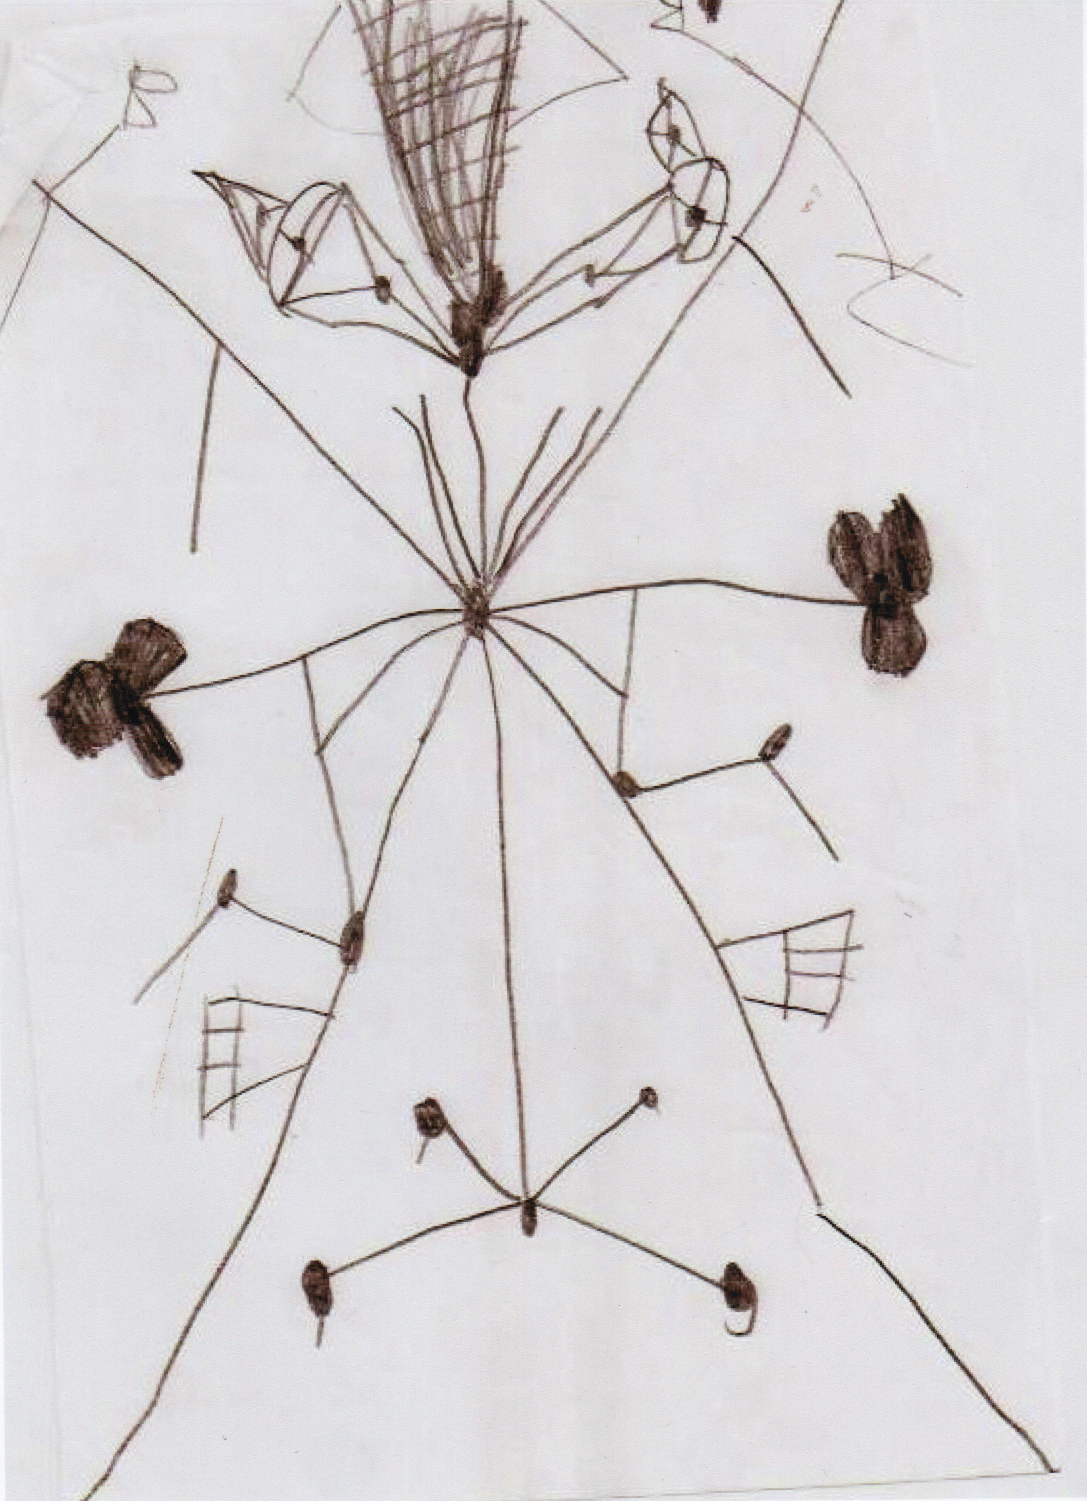
\includegraphics[scale=0.4]{robhootcartoon.pdf}
\end{center}
\caption{Our dream icon $\mathcal{ROBHOOT}$}
\end{figure}
\end{flushleft}

\newpage


\tableofcontents
\newpage

\section{Abstract}

High-resolution data coming from many sources is becoming standard in
many scientific fields. Yet, inferring insightful patterns and
processes integrating databases with analytical frameworks remain
challenging in many disciplines. In this work we aim to introduce the
main features of an automated workflow to integrate data, statistical
learning, AI algorithms and process-based models accounting for many
sources of bias to take better informed decisions in research,
management and investment landscapes.
\\
\\
Keywords: automated data integration, multilayer networks, approximate
Bayesian computation, process-based inference.
\newpage


\section{Introduction}

Achieving robustness and reproducibility in science is challenging
\citep{Ioannidis:2005}. One of its cornerstones is to achieve data
integration and insights from the processes that might govern the
patterns from such an integration to make testable predictions and to
facilitate new experiments. There are many bias and stages in the
scientific method that make such a data and insight integration hard
to follow. For example, sampling design and experiments, \index{robust
  algorithms} and randomizations to achieve solid statistics, model
selection and inference just to name a few. An ideal procedure might
account for all the bias integrating the minimal set of stages to
accomplish a given question (Figure 1 -- fully connected 5-layers and
an example).
\\

The main five components can be described as follows: 
...summarize here the 5 layers and why
\\


\section{Methods}

In this section we introduce each of the layers outlined in Figure
1. For any given question, there are different methods within each
layer that can complete the task. Ideally, one should be able to
choose the best method from each layer and connect them to reach
insightful patterns and predictions from the data. How many paths are
there? Which of these minimize bias? Which topology within and between
layers give the best response to our question?


\subsection{Data Collection and integration (DC)}

$\mathcal{DAAI}$ Package}

Data access platforms from genomes to ecosystems and markets of any
kind are highly scattered across the web
\footnote{\url{https://github.com/melian009/Robhoot/blob/master/resources/databases.md}}. This
means most interacting agents in the market have to deal with a highly
complex set of intermediate stages and regulations before having
access to the data. Having ``easy'' access to the information in a
``perfectly informed market'' should be simple and efficient, but
unfortunately, it is not. We aim to collect and clean data received
from different sources. The collected data can be available in CSV,
database, or "real time" (e.g. [Nakamoto
Terminal](https://www.nterminal.com), [BigQuery](
https://cloud.google.com/bigquery/)). We aim to have a package in
Julia language and let the user automatically get the data in their
desired format.

\subsection{Complexity Reduction (CR)}

$\mathcal{GOCORE}$ Package (Generalizing complexity reduction models)

PCA family -- High-dimensionality of Convex hull -- Information metrics multilayer networks\\


Data dimension reduction is a second step to increase performance
during the next stages of analysis.  Complexity reduction in economics
and in ecology has a long tradition mostly by looking at
variance-covariance matrices.  Portfolio theory in economics has a
long tradition \citep{MarkowitzBook}. The theory is rooted in the
concept of efficient frontier\index{efficient frontier}. There are
several packages in several languages to calculate efficient
frontiers\footnote{\url{http://www.quantcode.com/}}$^{,}$\footnote{\url{https://github.com/JuliaQuant/PortfolioModels.jl}}$^{,}$\footnote{\url{https://www.wikinvest.com/account/portfolio/register}}$^{,}$\footnote{\url{https://d1so5k0levrfcn.cloudfront.net/SigFig\%20Investment\%20Methodology.pdf}}. Most
maths underlying portfoliio theory\index{portfolio theory} are based
in matrix correlation patterns\index{matrix correlation patterns}. In
ecology, portfolio concept has also been used to predict the number of
coexisting species in landscapes with highly fluctuating
environments\footnote{Check references}.

Many fields aim at predicting fluctuations of several time series at
local and regional scales. The better the predictions are the better
we know the ecosystem. Unfortunately, it is not easy to predict time
series of a large number of interacting (ideally independent)
variables. Given we can not predict most of the ideas' trends, we
should build a minimum understanding on how to investigate ideas and
build a diversified portfolio with a balance between risk and
reward. Basic questions will always remain when discussing about
predicting the future and diversifying portfolios. For example, in a
complex ecosystem, which is the best strategy under complete
ignorance? And under complete information?  Should we invest in ideas
following a random walk \index{random walk}? Should we produce a
portfolio with neutral risk \index{neutral risk}?
\footnote{\url{https://en.wikipedia.org/wiki/A$_$Random$_$Walk$_$Down$_$Wall$_$Street}}. Given
the basic maths underlying complexity reduction, which are the
algorithms and models out there? Which one perform the best? Which is
the mixed of models to minimize data complexity?
\\

\subsection{Pattern Inference (PI)}

$\mathcal{PROPENCE}$ Package

Outline classical variance-covariance matrices, AI
algorithms and process-based methods.

\subsection{Model Validation (MV)}

$\mathcal{VATION}$

Describe briefly Bayesian Inference, Approximate Bayesian computation, AIC and BIC model comparison methods.
Gibbs sampling -- Bayes factors


\subsection{Visualization (VI)}


\subsection{Examples}

$\mathcal{ROBHOOT}$

In this section, we will use $\mathcal{ROBHOOT}$ to illustrate how it
works. $\mathcal{ROBHOOT}$ will be a semi-automated tool combining
access to data from both centralized and decentralized platforms and
integrating the datasets to infer insights and predictions obtained
from analyzing patterns in the datasets (Figure 1). We aim to develop
$\mathcal{ROBHOOT}$ in two stages. The first stage will be to develop
the free-access platform to have access to integrated databases. The
second stage will be to run it automatically to produce insights and
pattern inference given specific questions (Figure 1). 

\section{Discussion}


\newpage
\section{Acknowledgments}


\newpage
\bibliographystyle{evolution}
\bibliography{ref}

\newpage

\section{Tables}


\newpage

\section{Figures}

%Figure 1: Flowchart 1 5--fully connected layers and a example

%Figure 2: ROBHO0T: Steps to develop ROBHO0T
%\begin{figure}
%\vspace{-1 in}
%\begin{center}
%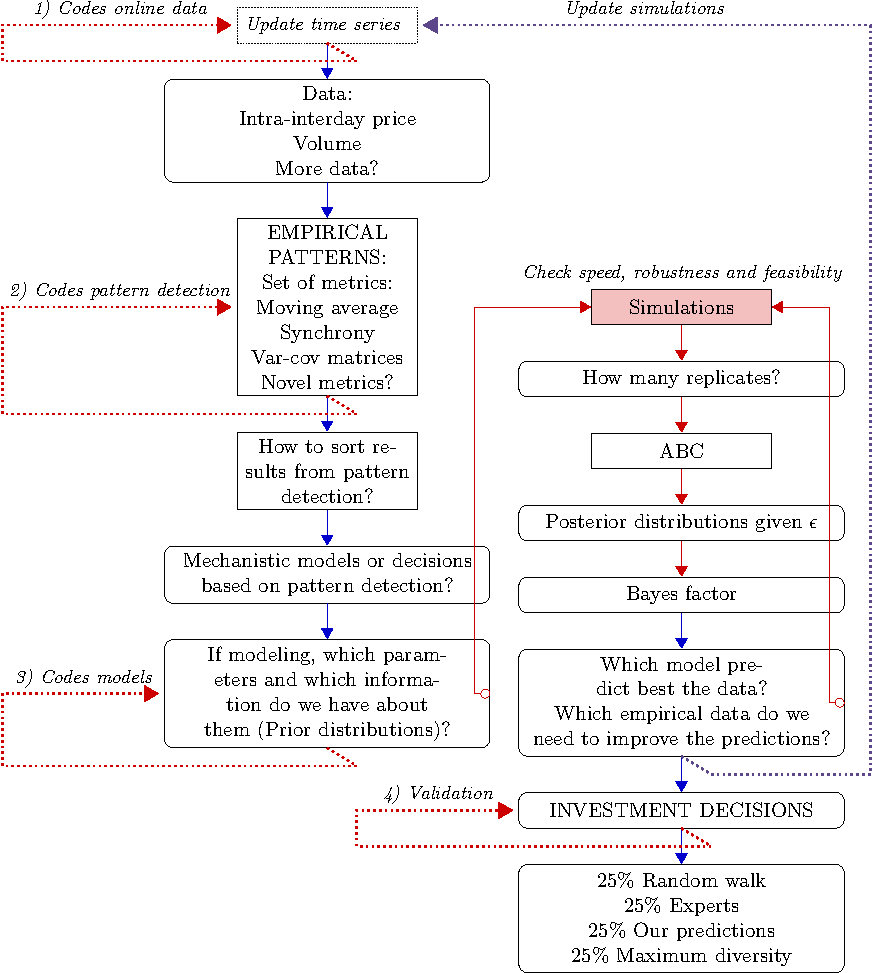
\includegraphics[scale=0.8]{EasyFlowChart.pdf}
%\end{center}
%\caption{Flow chart summarizing the steps to develop $\mathcal{ROBHOOT}$}
%\label{}
%\end{figure}
%\newpage

%Figure 3: ROBHOT: Steps to develop ROBHOT
%\begin{figure}
%\vspace{-1 in}
%\begin{center}
%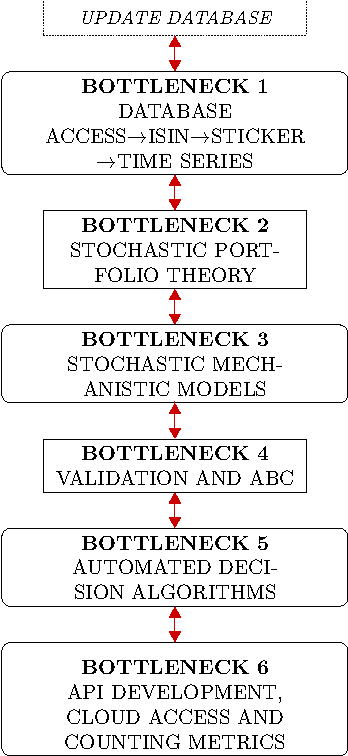
\includegraphics[scale=1.25]{EasyFlowChartBottlenecks.pdf}
%\end{center}
%\caption{Bottlenecks to overcome to develop $\mathcal{ROBHOOT}$}
%\end{figure}
%\newpage


\printindex
\end{document}
